\section{Конструкторская часть}
В данном разделе будут представлена IDEF0 диаграмма метода, схемы алгоритма и структура приложения. Описан формат входных и выходных данных.

\subsection{IDEF0 диаграмма}
На рисунках \ref{idef0:top} -- \ref{idef0:A3} представленна IDEF0 диаграмма.

\begin{figure}[h]
	\begin{center}
		{\includegraphics[scale=0.63, angle=-90, page=1]{img/idef0.pdf}}
		\caption{IDEF0, контекстная диаграмма А0}
		\label{idef0:top}
	\end{center}
\end{figure}

Разрабатываемый метод состоит из нескольких этапов, описанных на рисунке \ref{idef0:A0}. В первую строится опорный план грузоперевозок по модифицированному методу минимального элемента. Далее для него применяется также изменённый под условия решаемой задачи метод потенциалов. Результатом конечного числа итераций данного метода становится оптимальный набор маршрутов перевозки. По нему составляется расписание с использованием метода интервалов.

\begin{figure}[h]
	\begin{center}
		{\includegraphics[scale=0.63, angle=-90, page=2]{img/idef0.pdf}}
		\caption{IDEF0 диаграмма, декомпозиция А0}
		\label{idef0:A0}
	\end{center}
\end{figure}

Метод минимальных элементов описан с помощью диаграммы на рисунке \ref{idef0:A1}. Этот метод можно разделить на 3 действия. В первую очередь расчитываются кратчайшие расстояния пунктов с помощью алгоритма Дейкстры. Далее создаётся список всех маршрутов до каждого потребителя от стоянки через ближайшие склады. Последним этапом производится основное действие метода --- на маршруты в порядке возрастания их стоимости распределяется максимальное возможное количество грузов. 

Итогом этапа является опорный план грузоперевозок.

\pagebreak
\begin{figure}[h]
	\begin{center}
		{\includegraphics[scale=0.63, angle=-90, page=3]{img/idef0.pdf}}
		\caption{IDEF0 диаграмма, декомпозиция А1}
		\label{idef0:A1}
	\end{center}
\end{figure}

Следующий этап выполняет задачу оптимизацию плана перевозки и разделяется на четыре шага.
\begin{enumerate}
	\item Вычисление потенциалов осуществляется отдельно для каждого продукта, следуя по опорному плану. Результатом шага является матрица потенциалов --- значения стоимости доставки для каждого пункта по каждому товару.
	\item Вычисление невязок производится путём сравнения значения потенциалов в соседних пунктах. Полученные величины сохраняются в список.
	\item Производится рассмотрение всех невязок в порядке возрастания их величин. Изменением маршрутов формируется новый план.
	\item В следующем этапе полученный план сравнивается с опорным по функции стоимости. В случае её уменьшения создаётся новый опорный план и осуществляется новая итерация метода.
\end{enumerate}

\pagebreak
\begin{figure}[h]
	\begin{center}
		{\includegraphics[scale=0.63, angle=-90, page=4]{img/idef0.pdf}}
		\caption{IDEF0 диаграмма, декомпозиция А2}
		\label{idef0:A2}
	\end{center}
\end{figure}

В заключающем этапе формируется расписание. Для каждого маршрута подбирается время его начала, чтобы избежать одновременного обслуживания а пунктах вместе с другими маршрутами.

\pagebreak
\begin{figure}[h]
	\begin{center}
		{\includegraphics[scale=0.63, angle=-90, page=6]{img/idef0.pdf}}
		\caption{IDEF0 диаграмма, декомпозиция А3}
		\label{idef0:A3}
	\end{center}
\end{figure}

\subsection{Схемы алгоритмов}
На рисунках \ref{alg:main} - \ref{alg:schedule} представлены схемы ключевых алгоритмов программы.

\subsubsection{Основной алгоритм}
Весь алгоритм оптимизации изображён на рисунке \ref{alg:main}. Его можно выделить следующие основные этапы:
\begin{enumerate}
	\item Вычисление начального баланса продуктов.
	\item Составление опорного плана.
	\item Оптимизация плана.
	\item Формирование расписания.
\end{enumerate}

Рассмотрим упомянутые этапы подробнее в следующих схемах.

\pagebreak
\begin{figure}[h]
	\begin{center}
		{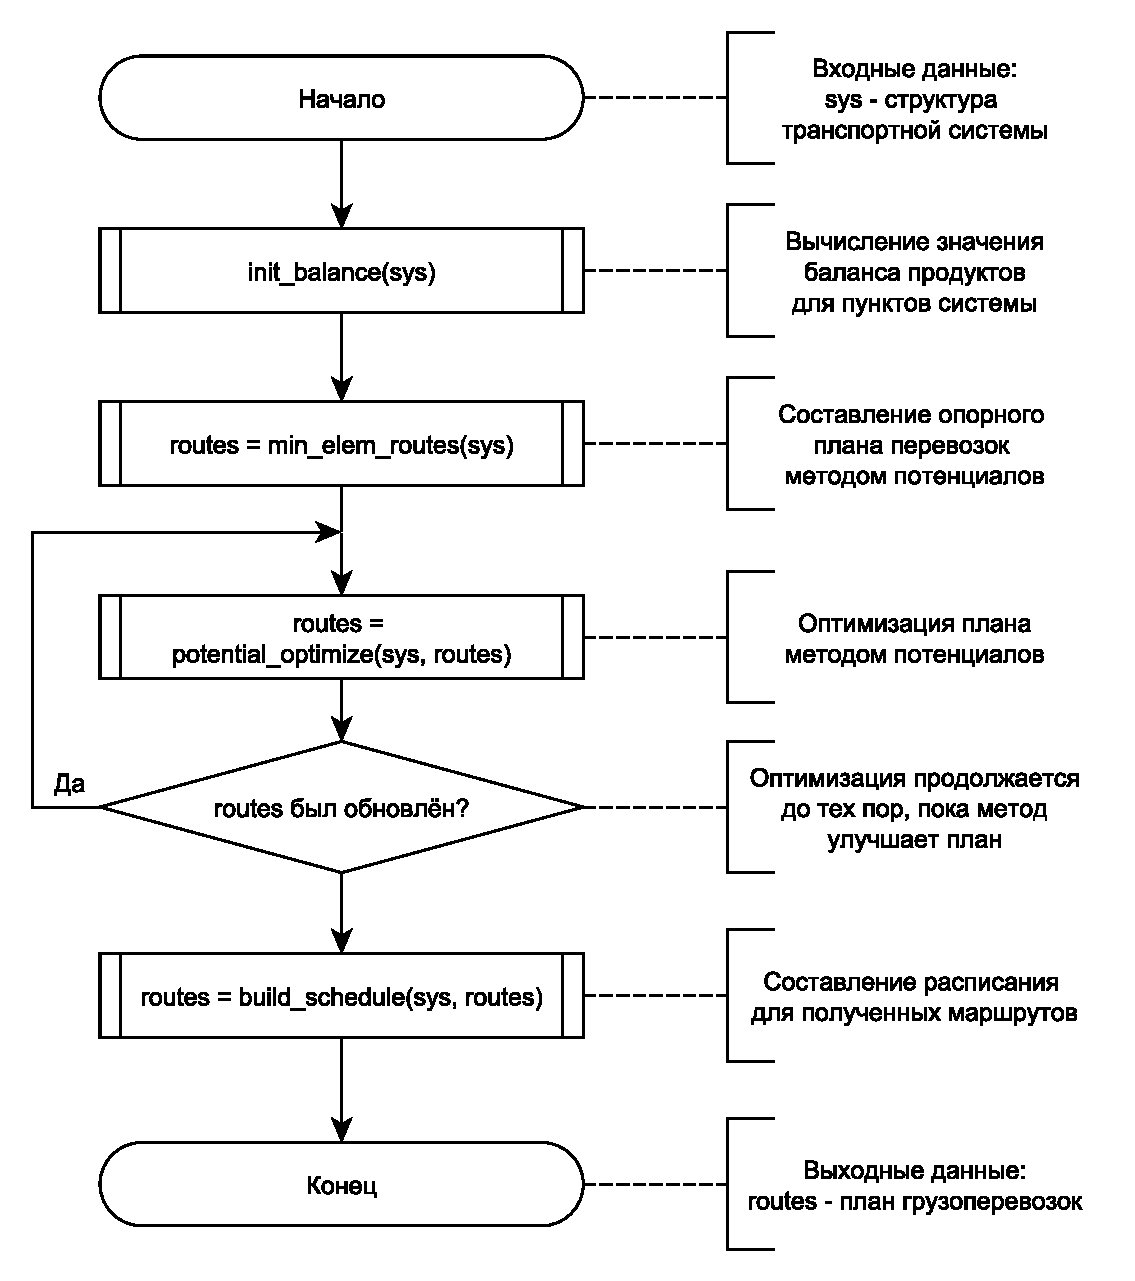
\includegraphics[scale=0.7, angle=0, page=1]{img/main_algorithm.pdf}}
		\caption{Схема общего алгоритма программы}
		\label{alg:main}
	\end{center}
\end{figure}

\subsubsection{Вычисление начального баланса}
При вычислении баланса, схема которого изображена на рисунке \ref{alg:balance}, для всех складов значение выставляется как количество хранимой продукции, для всех потребителей число заказанных тар продуктов со знаком минус. Баланс стоянки нулевой. Данный этап нужен для проверки соблюдения ограничения количества продукции в различных пунктах. 

\pagebreak
\begin{figure}[h]
	\begin{center}
		{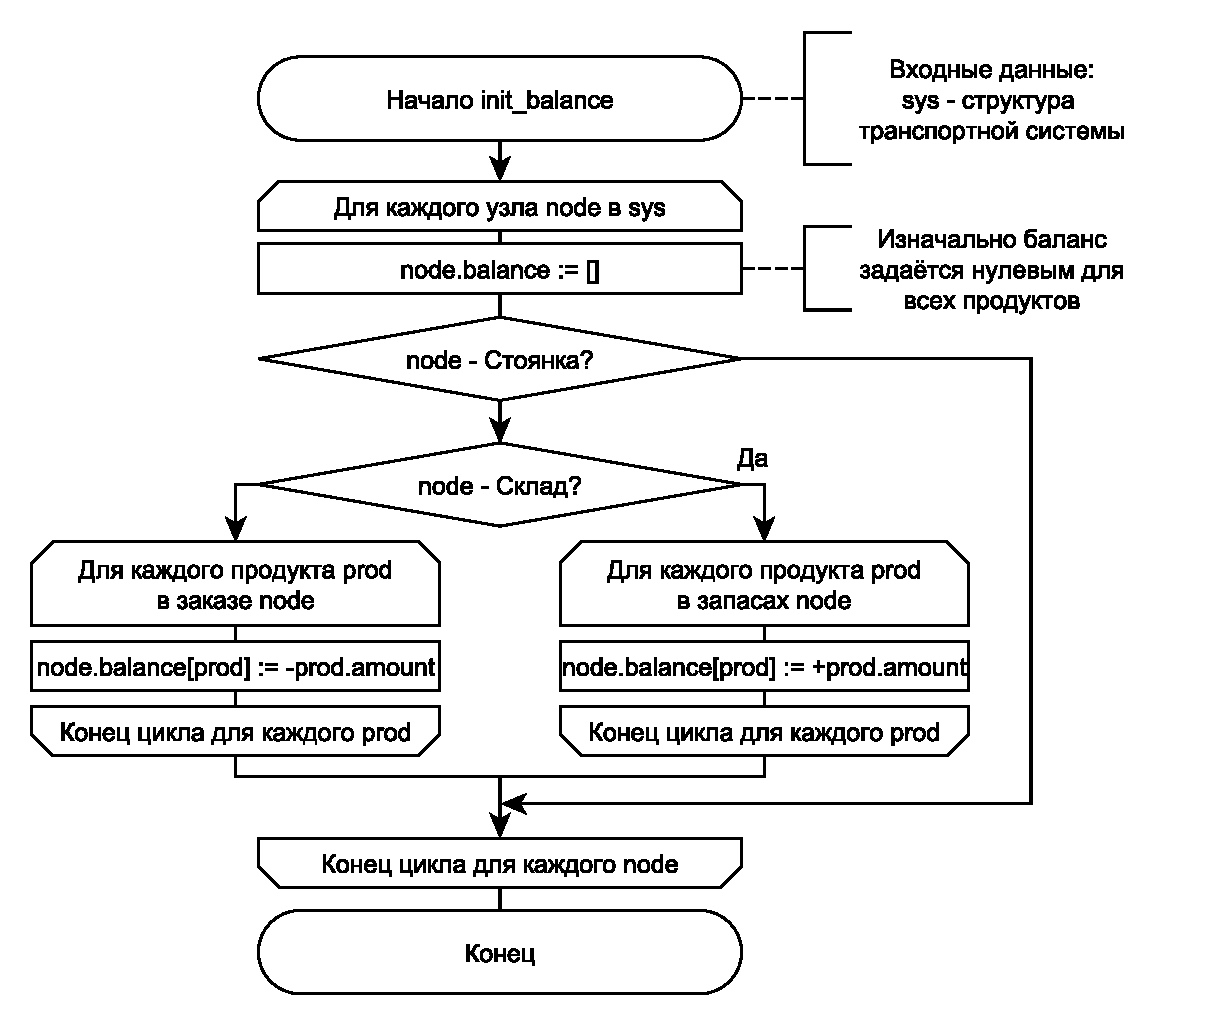
\includegraphics[scale=0.7, angle=0, page=1]{img/init_balance.pdf}}
		\caption{Схема алгоритма вычисления начального баланса}
		\label{alg:balance}
	\end{center}
\end{figure}

\subsubsection{Составление опорного плана}
На этом этапе формируется опорный план грузоперевозки. Для этого все маршруты, ведущие к каждому потребителю через склад по вычисленному кратчайшему пути, просматриваются в соответствии с методом минимального элемента --- в порядке возрастания их стоимости. 

\begin{figure}[hp]
	\begin{center}
		{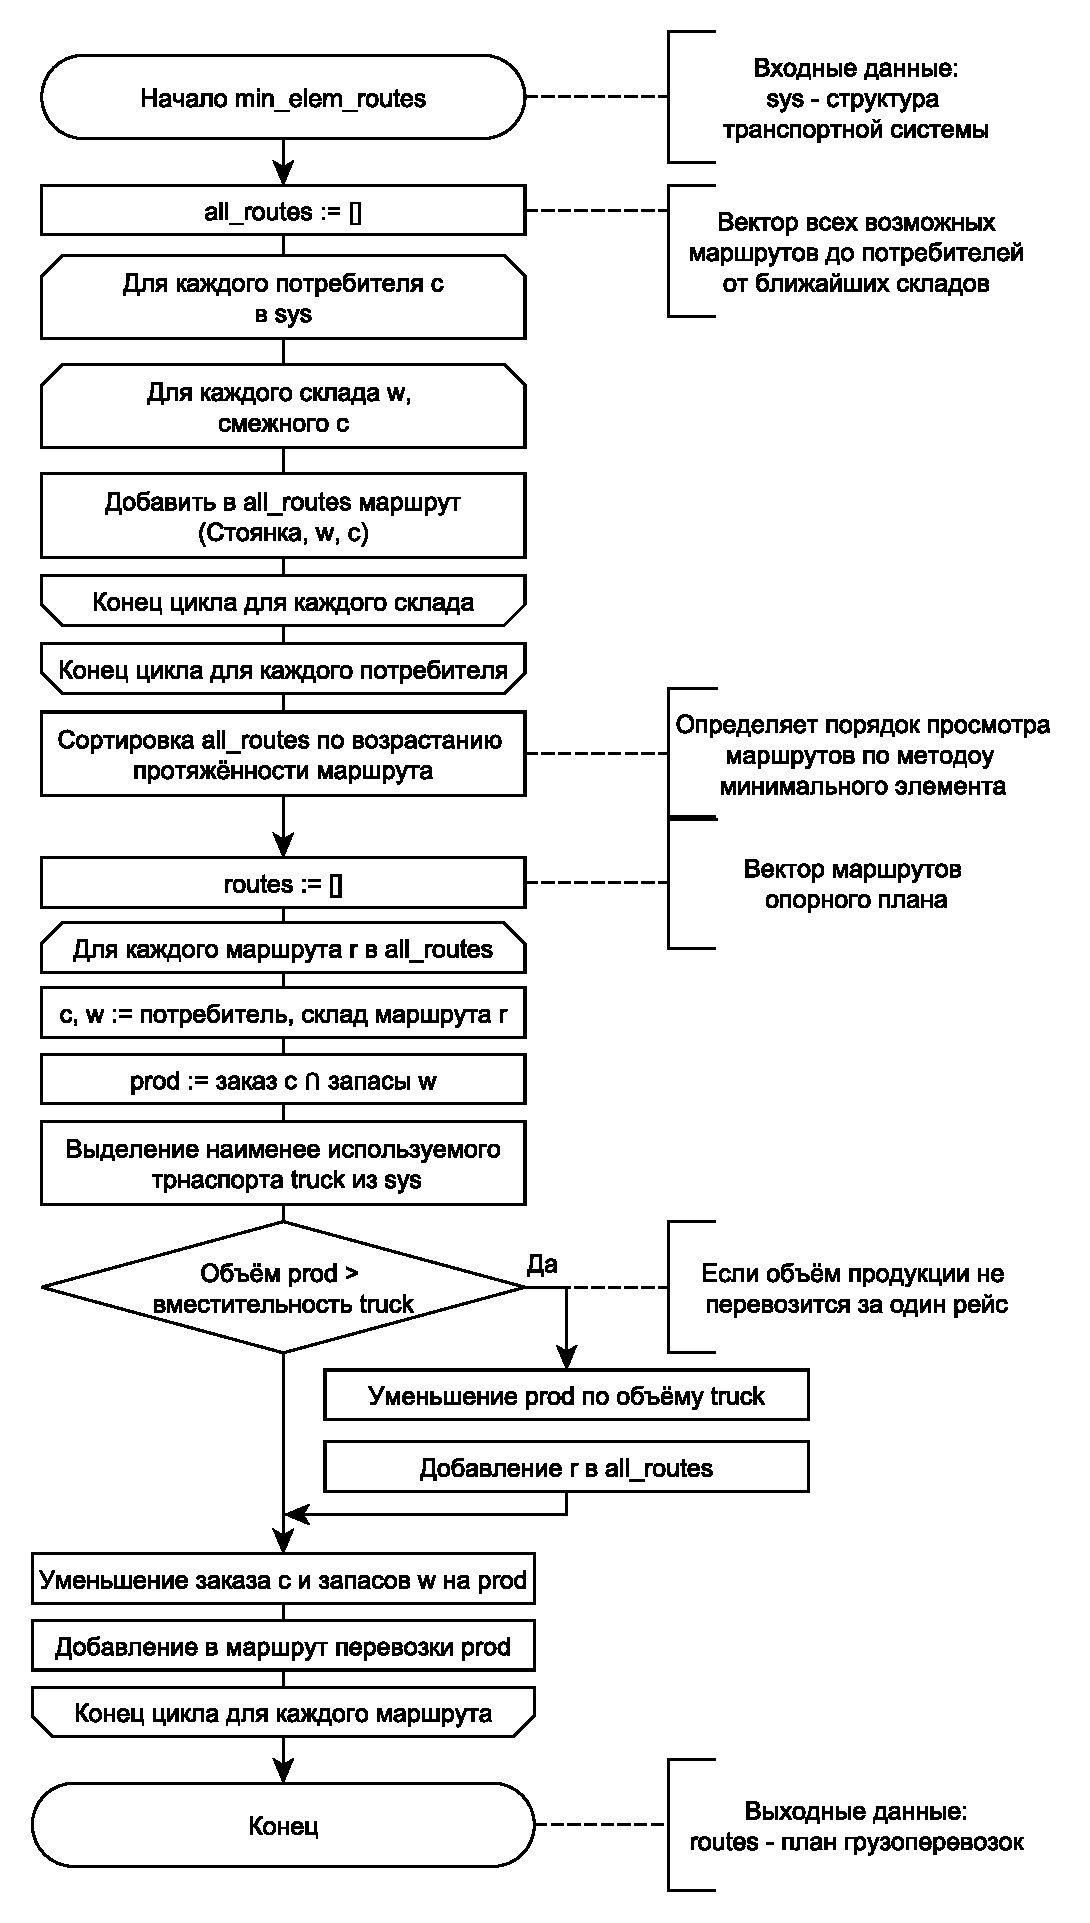
\includegraphics[scale=0.7, angle=0, page=1]{img/min_elem_routes.pdf}}
		\caption{Схема алгоритма минимального элемента}
		\label{alg:min_elem}
	\end{center}
\end{figure}

\subsubsection{Оптимизация плана}
Рисунки \ref{alg:potential_1} - \ref{alg:potential_2} описывают алгоритм оптимизации плана. После вычисления потенциалов начинается рассмотрение узлов, для которых обнаружены невязки. Анализируется возможность замены перевозки текущих маршрутов-поставщиков альтернативными, завершающимися на смежных пунктах. Другие маршруты продлеваются по очереди убывания их выгодности для данного пункта и по мере ограничений.

Если после замены оригинального маршрута в данном пункте функция стоимости для плана становится меньше, то изменения принимаются за новый опорный план. Иначе, поиск оптимизации продолжается далее.

\begin{figure}[h]
	\begin{center}
		{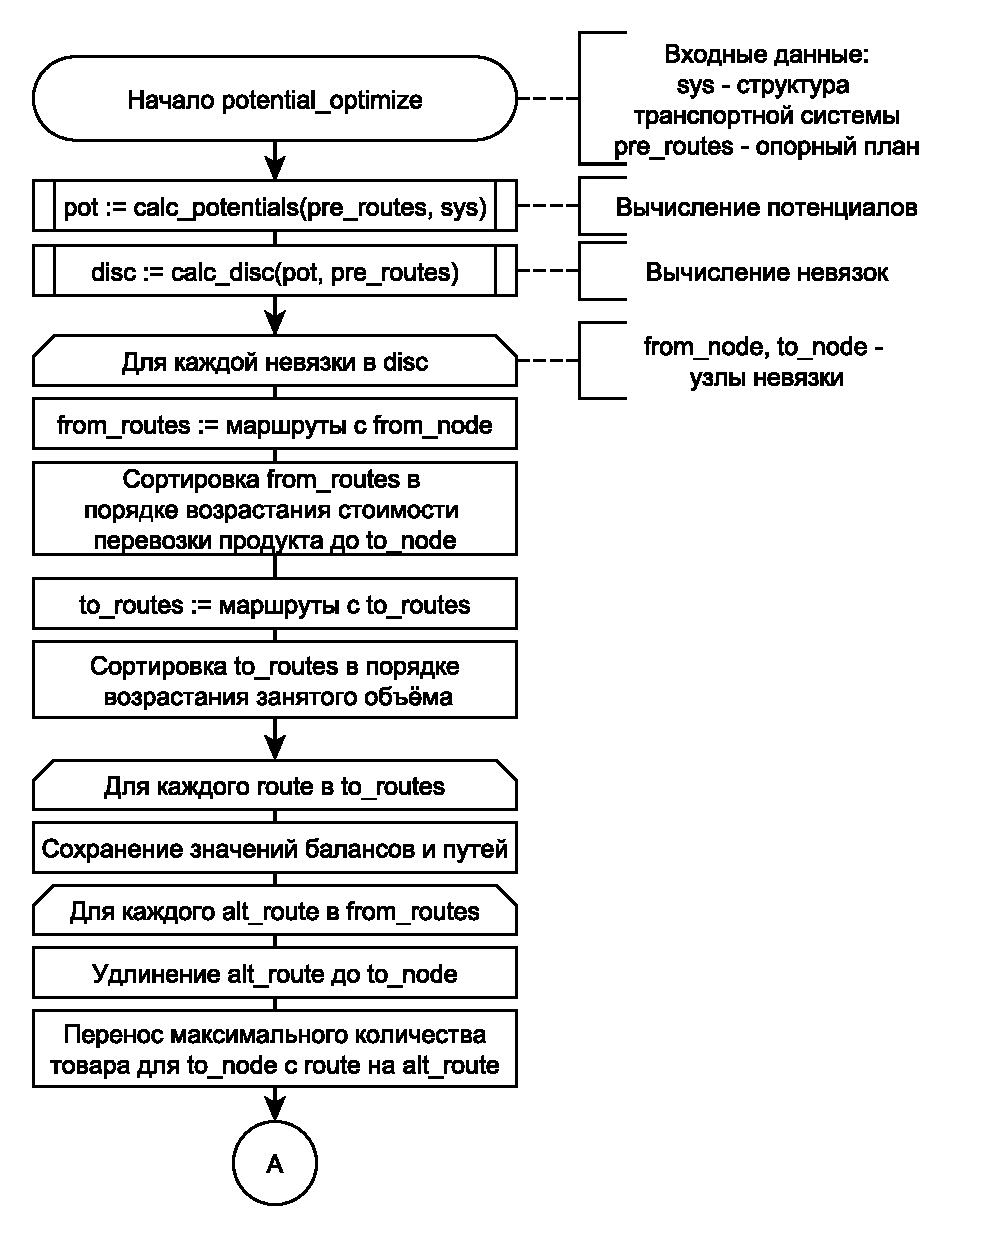
\includegraphics[scale=0.7, angle=0, page=1]{img/potential_optimize_1.pdf}}
		\caption{Схема алгоритма оптимизации методом потенциалов}
		\label{alg:potential_1}
	\end{center}
\end{figure}

\begin{figure}[h]
	\begin{center}
		{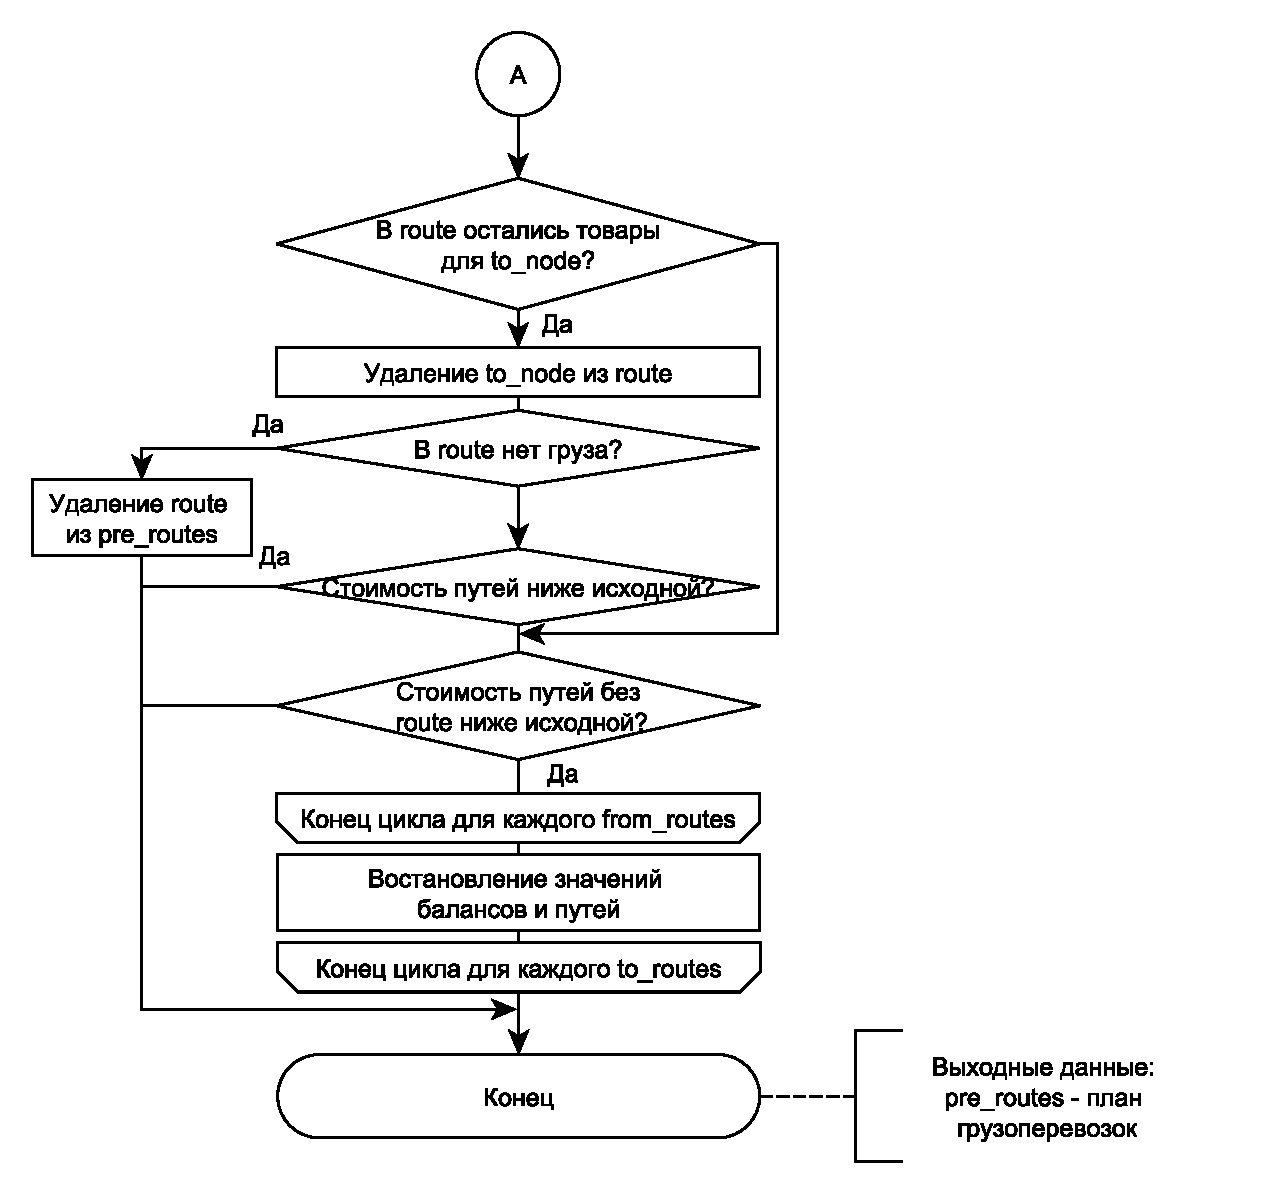
\includegraphics[scale=0.7, angle=0, page=1]{img/potential_optimize_2.pdf}}
		\caption{Схема алгоритма оптимизации методом потенциалов (продолжение)}
		\label{alg:potential_2}
	\end{center}
\end{figure}

\subsubsection{Формирование расписания}
Рисунок \ref{alg:schedule} описывает алгоритм формирования расписания. Изначально все маршруты выставляются на начало работы. В соответствии с описанными в системе продолжительностями проезда по дорогам и временами обслуживания в пунктах, формируется время прибытие и отбытия из каждого пункта маршрута. 

Далее осуществляется поочерёдное рассмотрение расписаний маршрутов, если оно не пересекается с уже принятыми, то маршрут добавляется в общее расписании с закреплением транспорта. Пересечением называется остановка на одном пункте в одинаковый промежуток времени. Величиной пересечения является общее время нахождения на пункте.

\begin{figure}[hp]
	\begin{center}
		{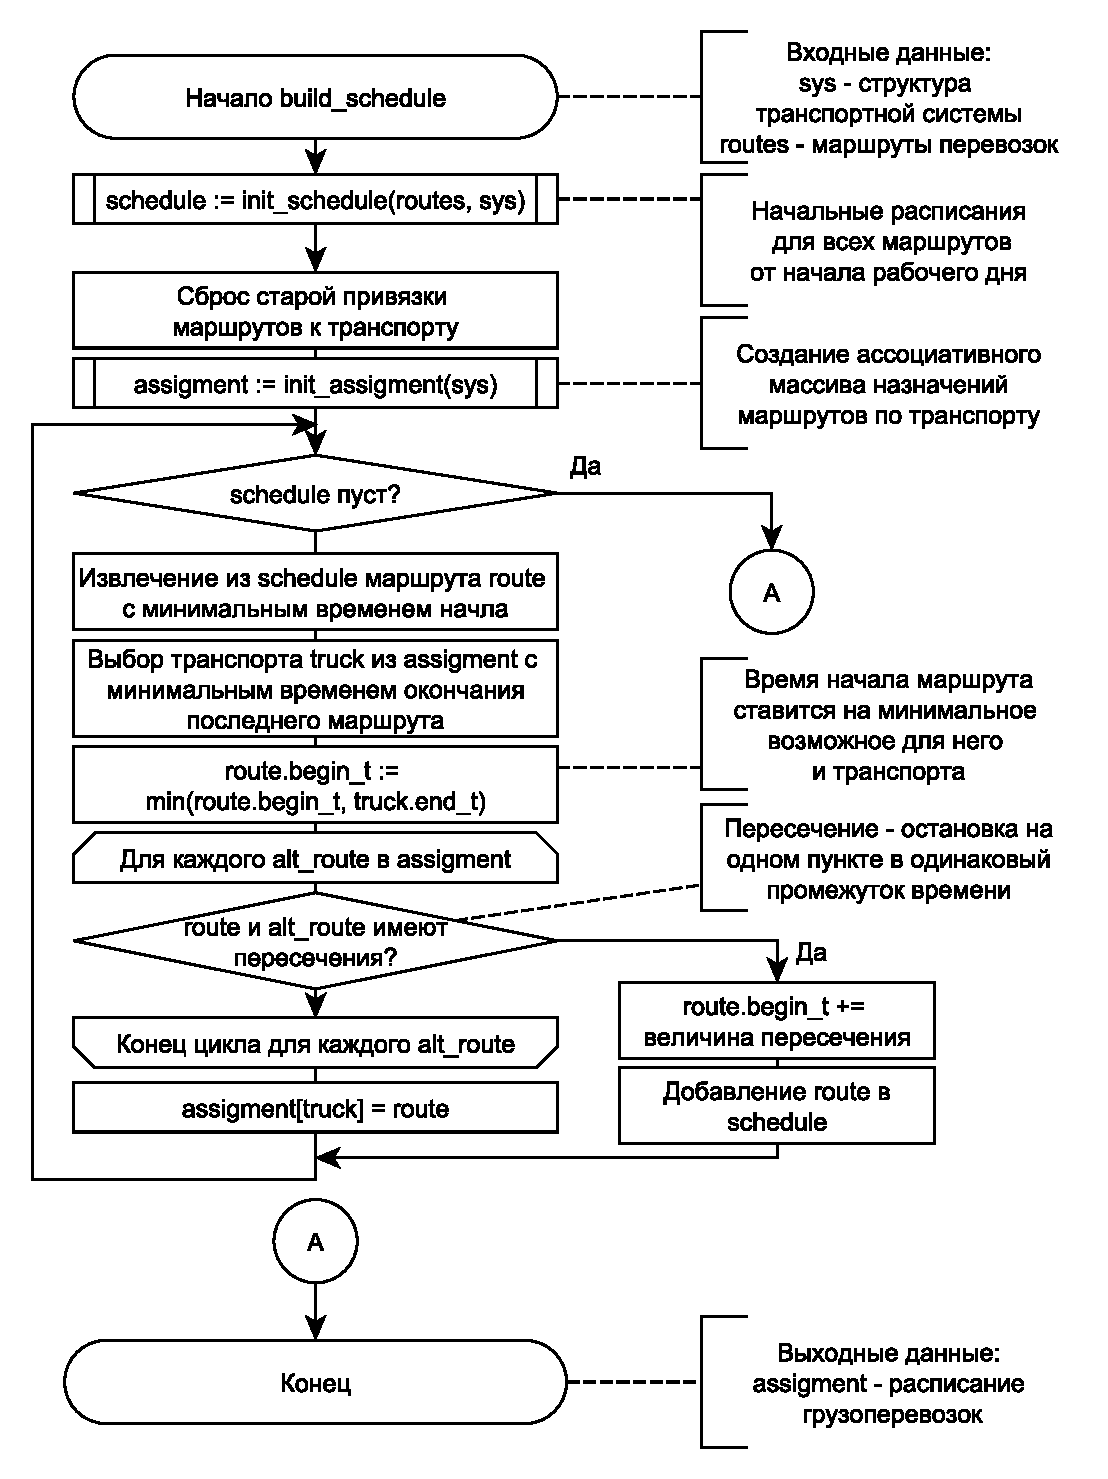
\includegraphics[scale=0.7, angle=0, page=1]{img/schedule.pdf}}
		\caption{Схема алгоритма составления расписания}
		\label{alg:schedule}
	\end{center}
\end{figure}

\subsection{Схема сущностей транспортной системы}
В соответствии с ранее описанной математической моделью, в системе должны быть представлены сущности, изображённые на рисунке \ref{ER} ER-диаграммой.

\begin{figure}[h]
	\begin{center}
		{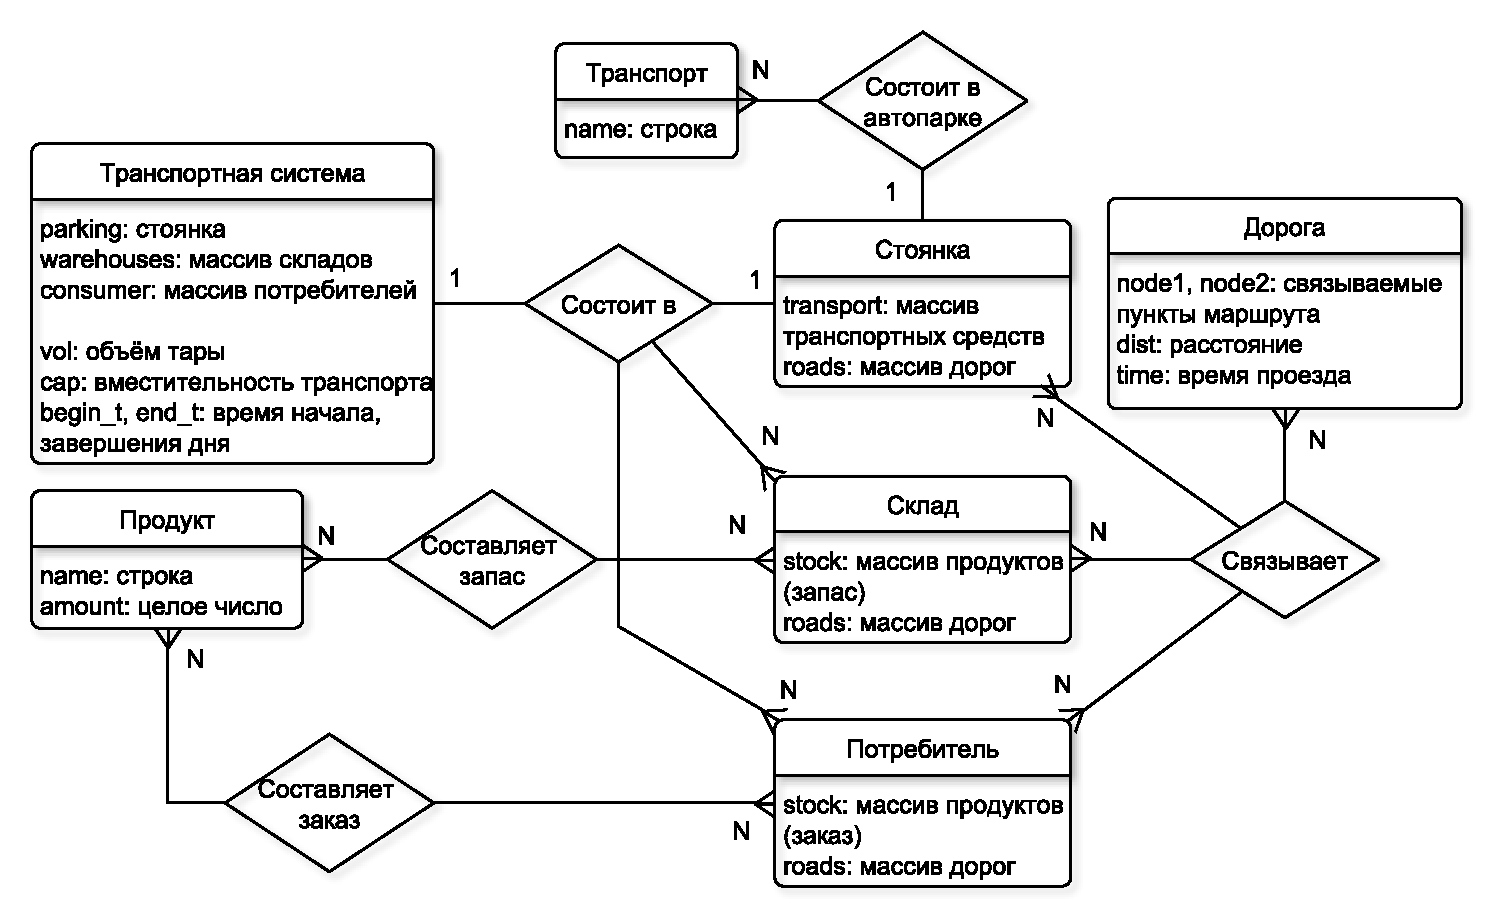
\includegraphics[scale=0.7, angle=0, page=1]{img/ER.pdf}}
		\caption{ER-диаграмма}
		\label{ER}
	\end{center}
\end{figure}

\pagebreak
\subsection{Формат входных данных}
В качестве входных данных выступает описание транспортной системы. Оно должно содержать в себе следующую информацию:

\begin{itemize}
	\item Список всех пунктов маршрута.
	\item Вместительность (в м$^3$) и количество транспорта.
	\item Список запасов складов. Каждый склад описывается списком продуктов (название и количество тар).
	\item Список заказов потребителей -- аналогично запасам складов.
	\item Список дорог: два связанных пункта, расстояние (в км.), время проезда (в мин.).
	\item Объём одной тары в (в м$^3$).
	\item Время начала и завершения рабочего дня.
\end{itemize}

\subsection{Формат выходных данных}
В качестве выходных данных выступает описание плана грузоперевозок. Оно состоит из списка маршрутов, каждый из которых должен содержать в себе следующую информацию:

\begin{itemize}
	\item Последовательность посещения пунктов.
	\item Номер привязанного транспортного средства.
	\item Список товаров, загружаемых или выгружаемых на каждом пункте.
	\item Список времени прибытия и отбытия в каждый пункт маршрута.
\end{itemize}	

\subsection*{Вывод}
В данном разделе были представленны IDEF0 и ER диаграммы, схемы алгоритмов. Описан формат входных и выходных данных программы.

\pagebreak